\documentclass[a4paper]{article}

\usepackage[T2A]{fontenc}
\usepackage[utf8]{inputenc}
\usepackage[russian, english]{babel}
\usepackage{amsmath, amsfonts, amssymb, amsthm, mathtools}
\usepackage{graphicx}
\usepackage{wrapfig}
\usepackage[rgb]{xcolor}
\usepackage{hyperref}
\usepackage{multirow}
\hypersetup{colorlinks=true, urlcolor=blue}

\author{Филохин Григорий\\Б04-106}
\title{Лабораторная работа 3.3.1\\Измерение удельного заряда электорна методами магнитной индукции}
\date{\today}


\begin{document}

\maketitle
\newpage

\section*{Цель работы}
Определение отношения заряда эдектрона к его массе методом магнитной фокусировки и методом магнетрона.

\section*{Оборудование}
\subsection*{Установка А}
Электронно-лучевая трубка (с блоком питания), соленоид, регулируемый источник постоянного тока, вольтметр,
магнитометр (милливеберметр).
\subsection*{Установка Б}
Электронная лампа с цилиндрическим анодом, регулируемый источник постоянного тока,
соленоид, вольтметр, два амперметра.


\section*{Метод магнитной фокусировки}

\subsection*{Теоретическая справка}

\begin{wrapfigure}{l}{4cm}
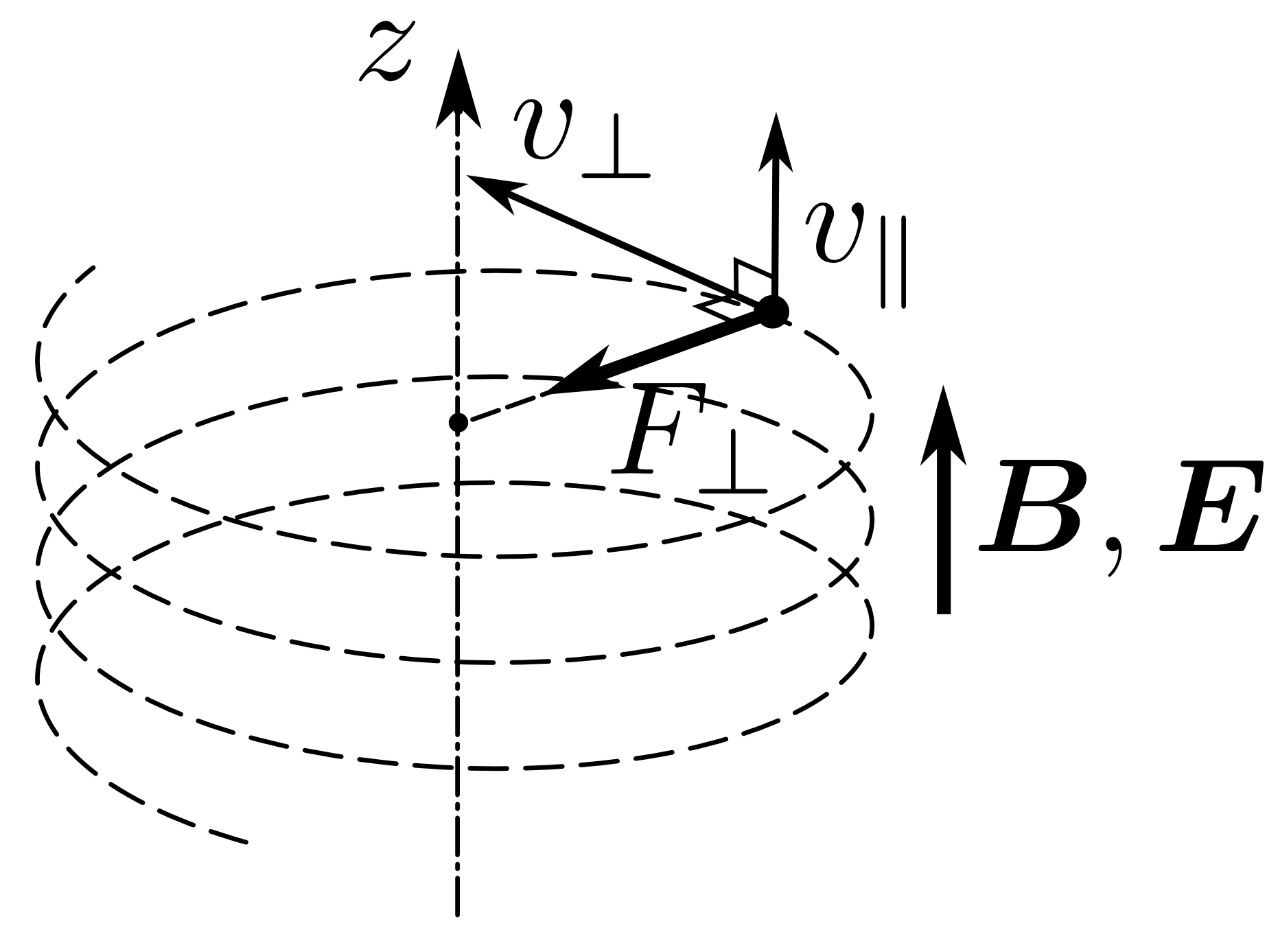
\includegraphics[width = 4cm]{Траектория}
\caption{Траектория в параллельных полях}
\end{wrapfigure}
В постоянном однородном магнитном поле траектории заряжен­ных частиц представляют собой спирали, радиус которых определя­ется формулой

\begin{align}
	r = \dfrac{m \upsilon_\perp}{q B}
\end{align}

За время $T_B = \dfrac{2\pi r}{\upsilon_\perp}$(циклотронный период) заряд сместится вдоль магнитного поля на расстояние (шаг спирали)
\[L = \upsilon_\parallel T_B = \dfrac{2\pi \upsilon \cos{\alpha}}{\frac{e}{m}B},\]
где $\alpha - $ угол между вектором скорости $\upsilon$ и направлением поля $B$. Если углы малы, то $\cos{\alpha}\approx 1$ и 

\begin{align}\label{spiral step}
	L \approx \frac{2\pi\upsilon}{\frac{e}{m} B}
\end{align}

Таким образом, при малых углах расстояние $L$ не зависит от $\alpha$, так что все электроны, вышедшие из одной точки, после одного оборота вновь соберутся в одной точке — сфокусируются. Как следует из \hyperref[spiral step]{(\ref{spiral step})}, индукция поля $B$ при которой точка фокусировки отстоит от точки вылета на расстоянии $L$ определяется величиной $\frac{e}{m}$ -- удельным зарядом частицы.

\subsection*{Установка}
Основной частью установки является электронный осциллограф, трубка которого вынута и установлена в длинном соленоиде, создающем магнитное поле, направленное вдоль оси трубки. Вылетая с катода, элек­троны имеют разные начальные скорости, соответствующие тепловой энергии $\sim 0.1$эВ. Затем эмитированные катодом электроны ускоряются большой анодной разностью потенциалов $U_A \sim 1$кВ и пропускаются через две диафрагмы, благодаря чему получается пучок частиц с малой расходимостью $\Delta\alpha \ll 1$ и малым разбросом продольных скоростей около значения
\[\upsilon_\parallel=\sqrt{\frac{2eU_A}{m}},\]следующего из ЗСЭ.

В магнитном поле соленоида %коллимированные
электроны будут двигаться по спиралям практически с одним и тем же шагом $L$ и, следовательно, будут встречаться вновь, пересекая ось пучка на расстояниях $nL, n = 1, 2, \ldots$. В этих точках сечение пучка будет наименьшим, и при изменении магнитного поля изображение пучка на экране будет периодически стягиваться в ярко светящуюся точку. Таким образом, удельный заряд может быть получен из соотношения

\begin{align}\label{RelativeMass}
\frac{e}{m} = \frac{8\pi^2U}{L^2}\cdot\frac{n^2}{B^2_{\text{Ф}}(n)}
\end{align}

Эта формула и лежит в основе экспериментального измерения удельного заряда электрона методом магнитной фокусировки.\\
Анодное напряжение, определяющее продольную скорость электро
нов, измеряется вольтметром. Магнитное поле в соленоиде создаётся по
стоянным током (\hyperref[MethMagnInduction]{fig. 2}), величина которого задаётся источником пита
ния постоянного тока и измеряется амперметром $A$ источника. Ключ К
служит для изменения направления поля в соленоиде.

\begin{figure}[h]
\begin{center}
	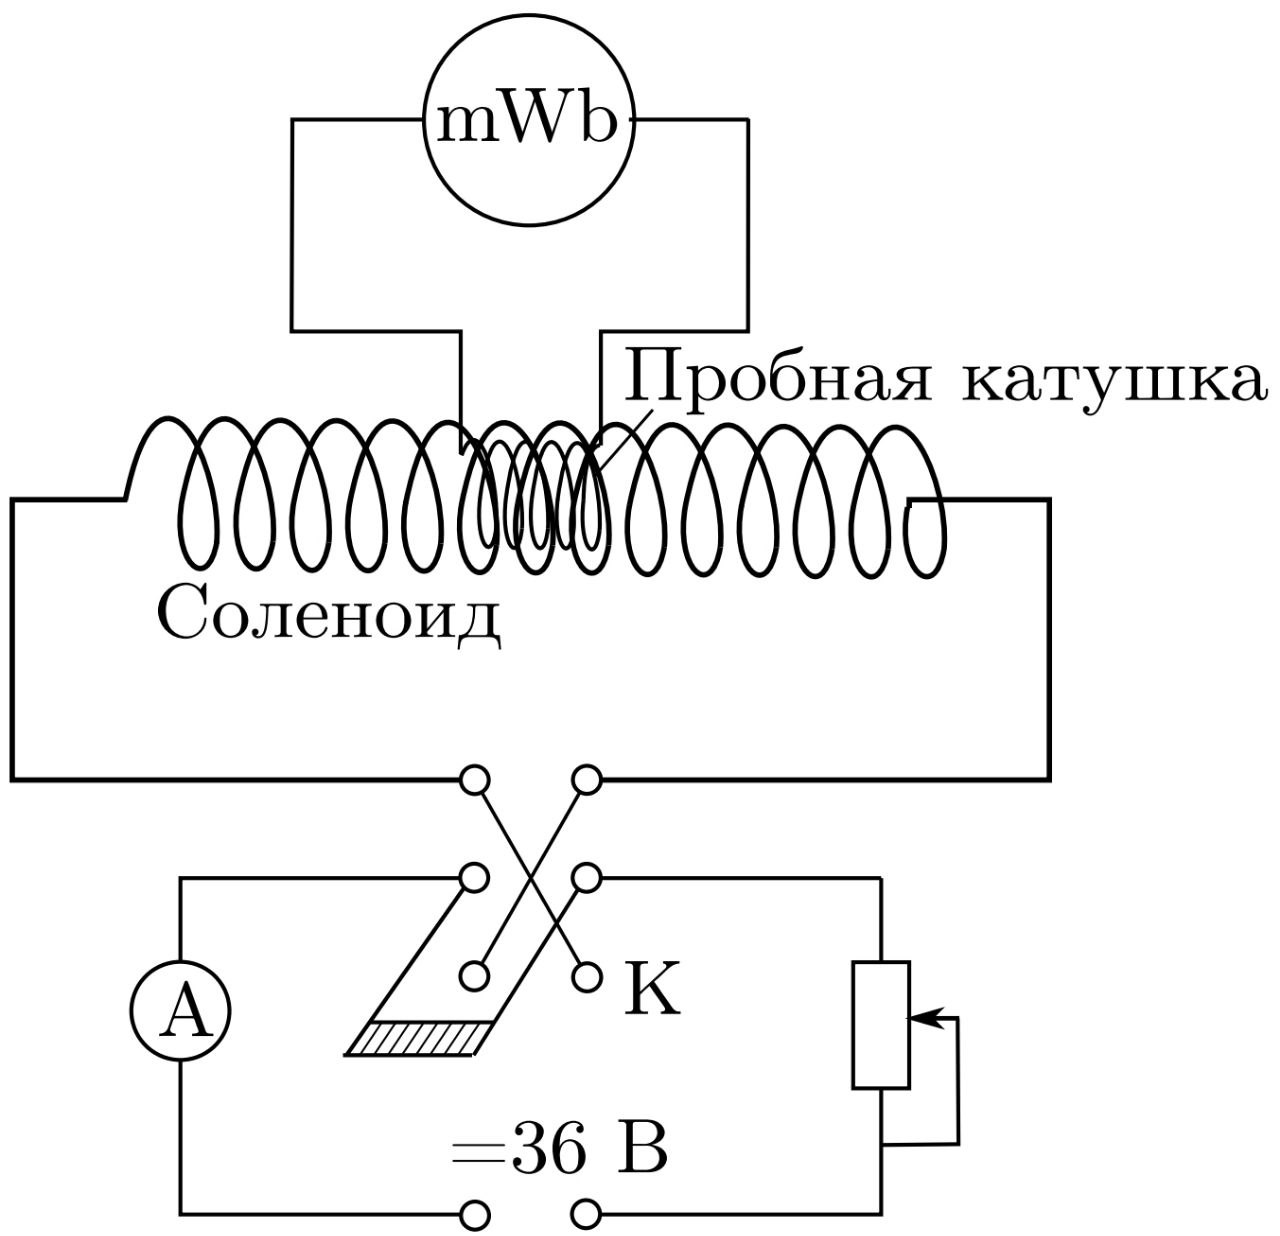
\includegraphics[width = 0.5\textwidth]{УстМагнФокусировки}
	\caption{Устоновка для метода магнитной фокусировки}
\label{MethMagnInduction}
\end{center}
\end{figure}

Величина магнитного поля определяется с помощью магнитометра, датчик которого расположен внутри соленоида. В качестве магнито­метра может использоваться милливеберметр. Датчиком милливеберметра является измерительная катушка, намотанная на один каркас с соленоидом. Таким образом измеряется изменение магнитного потока, пронизывающего измерительную катушку.\\
На точность результатов может влиять внешнее магнитное поле, осо­бенно продольное. Оно не вызывает размытия фокуса, но изменяет ве­личину фокусирующего поля. Присутствие внешнего магнитного поля проще всего обнаружить с помощью переполюсовки соленоида: при изме­нении направления поля показания милливеберметра будут отличаться, но их полусумма не зависит от наличия постоянного продольного поля.\\
Измерение магнитного поля производится в предварительных опы­тах: при отключённом ключе $K$ устанавливается связь между силой то­ка, протекающего через соленоид, и индукцией магнитного поля в соле­ноиде. По измеренным значениям строится калибровочный график $B(I)$, который используется при обработке результатов основных измерений
для определения индукции магнитного поля по известному току.

\subsection*{Эксперементальные данные}

Параметры установки:
\begin{align*}
SN & = 3000 \text{см}^2 & \sigma_I = & 0.07\text{А}\\
L & = 26.5 \text{см} & \sigma_{\textit{Ф}} = &  0.05 \text{мВб}\\
V & = 0.78 \text{кВ} & \sigma_V = & 10 \text{В}
\end{align*}

\begin{table}[h]
\begin{center}
\caption{Данные для калибровочной кривой B(I)}
\begin{tabular}{|c|c|c|}
\hline 
\textit{Ф}, мВб & $I$, А & $B$, мТл \\ 
\hline 
0.8 & 0.3 & 2.60 \\ 
\hline 
1.2 & 0.6 & 3.83 \\ 
\hline 
1.7 & 0.9 & 5.50 \\ 
\hline 
2.0 & 1.2 & 6.67 \\ 
\hline 
2.5 & 1.5 & 8.17 \\ 
\hline 
2.8 & 1.8 & 9.33 \\ 
\hline 
3.2 & 2.1 & 10.67 \\ 
\hline 
3.6 & 2.4 & 12.00 \\ 
\hline 
4.0 & 2.7 & 13.03 \\ 
\hline 
4.4 & 3.0 & 14.67 \\ 
\hline 
4.9 & 3.6 & 16.33 \\ 
\hline 
\end{tabular} 
\end{center}
\end{table}

\begin{figure}[h]
\begin{center}
	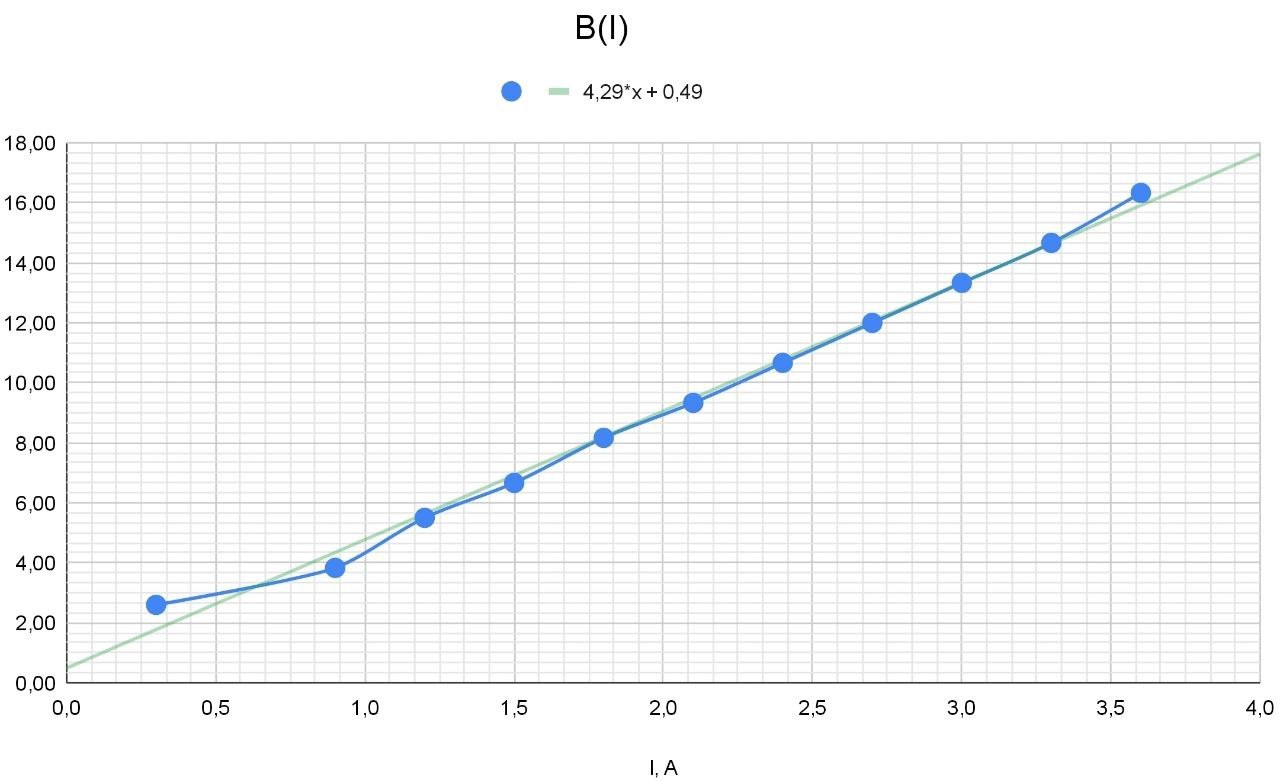
\includegraphics[width = 1.1\textwidth]{B(I)}
	\caption{График $B(I)$}
\end{center}
\end{figure}

Уравнение прямой: $y = 4.29x + 0.49$, значит будем искать $B_{\text{Ф}_n}$ по формуле:
\[B_{\text{Ф}_n} = 4.29 \cdot I_{\text{Ф}_n} + 0.49\]

\begin{table}
\begin{center}
\caption{Поиск вектора магнитной индукции, когда поток сфокусирован}
\begin{tabular}{|c|c|c|c|}
\hline 
Направление & $I_{\text{Ф}_n}$, А & $n$ & $B_{\text{Ф}_n}$, мТл \\ 
\hline 
\multirow{6}{*}{1} & 0.54 & 1 & 2.81 \\ 
\cline{2-4}
 & 1.09 & 2 & 5.17 \\ 
\cline{2-4}
 & 1.97 & 3 & 8.94 \\ 
\cline{2-4}
 & 2.27 & 4 & 10.23 \\ 
\cline{2-4}
 & 2.73 & 5 & 12.20 \\ 
\cline{2-4}
 & 3.19 & 6 & 14.18 \\ 
\hline 
\multirow{6}{*}{2} & 0.55 & 1 & 2.85 \\ 
\cline{2-4}
 & 1.10 & 2 & 5.21 \\ 
\cline{2-4}
 & 1.67 & 3 & 7.65 \\ 
\cline{2-4}
 & 2.21 & 4 & 9.97 \\ 
\cline{2-4}
 & 2.73 & 5 & 12.20 \\ 
\cline{2-4}
 & 3.17 & 6 & 14.09 \\ 
\hline 
\end{tabular} 
\end{center}
\end{table}

\begin{figure}[h]
\begin{center}
	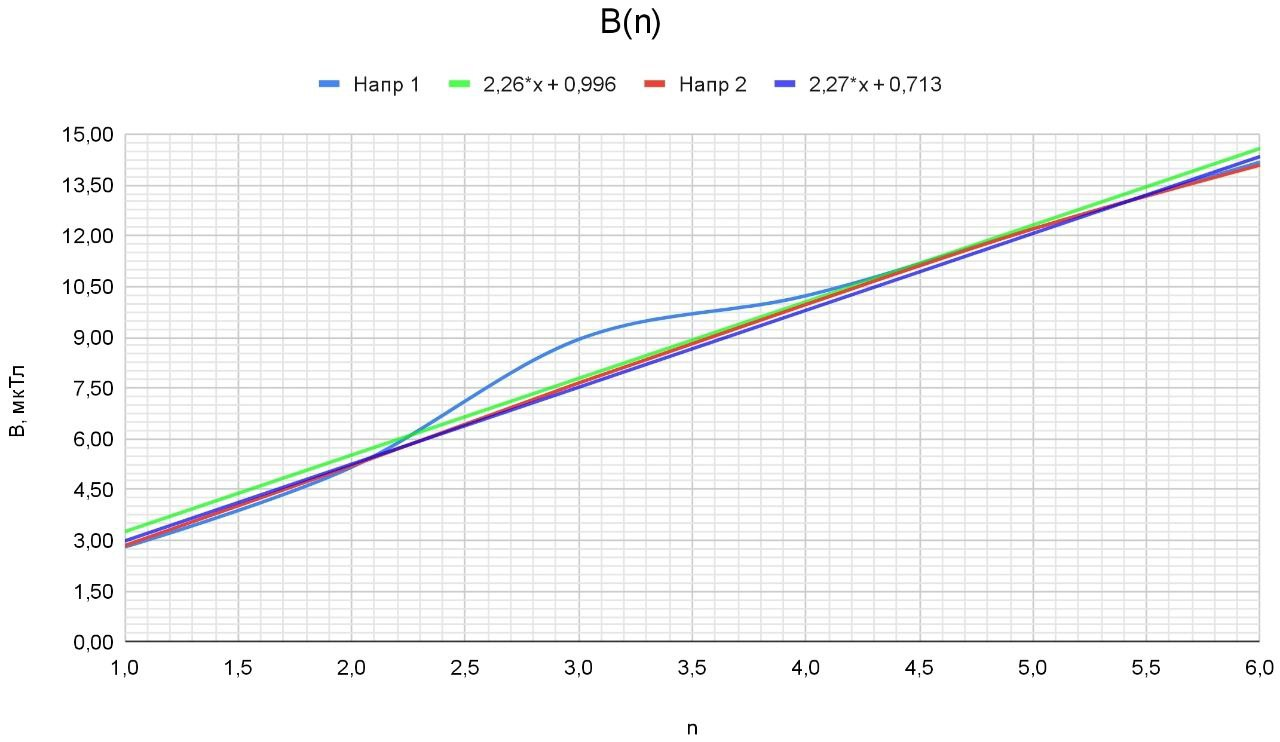
\includegraphics[width = \textwidth]{B(n)}
	\caption{График $B(n)$}
\end{center}
\end{figure}

Из графика $a_1 = 2.26, a_2 = 2.27$.\\
С помощью этих коэффициентов находим $\dfrac{e}{m}$ из формулы \hyperref[RelativeMass]{(\ref{RelativeMass})},где $\frac{n}{B_{\text{Ф}_n}} = \frac{10^3}{a_i}$.\\
\[W := \frac{8\pi^2V}{L^2} \approx 8.77 \cdot10^5\]
\[\frac{e}{m}_1 = \frac{W}{a_1} \approx 1.72 \cdot 10^{11}\hspace{2cm}\frac{e}{m}_1 = \frac{W}{a_2} \approx 1.70 \cdot 10^{11}\]


\clearpage
\section*{Метод магнитрона}
\subsection*{Теоретическая справка}
В методе магнетрона отношение $\frac{e}{m}$ измеряется на основе исследования движения электрона в скрещенных электрическом и магнитном полях. Название метода связано с тем, что такая конфигурация полей реализуется в магнетро­нах -- генераторах электромагнитных колебаний сверхвысоких частот.\\
Рассмотрим движение заряда $q$ во взаимно перпендикулярных однородных электрическом и магнитном полях $E\perp B$.\\
Уравнение движения заряда в таком случае имеет вид
\[m\dot{\upsilon} = qE + q\upsilon\times B.\]
Направим ось $z$ вдоль $B$, а ось $y$ -- вдоль $E$. Тогда, разделив на $m$, получим:
\begin{equation}\label{cycloid}
\begin{aligned}
	&\dot{\upsilon}_x = \omega_B \upsilon_y&\\
	&\dot{\upsilon}_y = \frac{q}{m}E - \omega_B \upsilon_x&\\
	&\dot{\upsilon}_z = 0&
\end{aligned}
\end{equation}

\begin{figure}[h]
	\begin{center}
		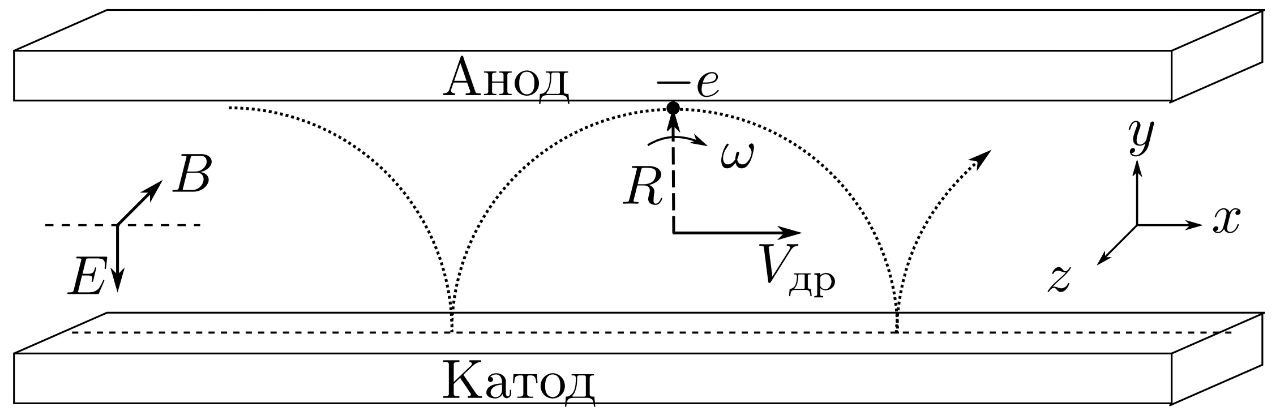
\includegraphics[width = \textwidth]{ДвижВСкрещПолях}
		\caption{Движение заряда в скрещенных полях}
	\end{center}
\end{figure}

Теперь рассмотрим упрощённую задачу о движении заряда в «плоском магнетроне». Пусть имеется
плоский конденсатор, в пространстве между пластинами которого со­здан высокий вакуум. Поместим его в однородное
магнитное поле так, что $E\perp B$. При этом отрицательная пластина конденсатора играет роль катода,
положительная — анода. Если бы магнитного поля не было, то все электроны, вылетевшие без начальной скорости из катода, попадали бы наанод. При наличии же магнитного поля траектории электронов искривляются, вследствие чего при достаточно большом $B$ ни один электрон не достигнет анода. Таким образом, при заданном напряжении $V$ между
пластинами существует некоторое критическое значение магнитной индукции $B_{\text{кр}}(V)$, при котором траектории касаются поверхности анода. Если  $B<B_{\text{кр}}$, то все электроны достигают анода, и ток через магнетрон
имеет то же значение, что и без магнитного поля. Если же $B>B_{\text{кр}}$, то электроны не достигают анода, и ток через вакуумный диод равен нулю.\\
Рассчитаем критическое магнитное поле для плоского конденсатора. Движение электрона будет иметь характер электрического дрейфа. Если начальная скорость равна нулю (начальные условия $x(0) = y(0) = 0, \upsilon_x(0) = \upsilon_y(0) = 0$), то, как следует из уравнений \hyperref[cycloid]{(\ref{cycloid})}, траектория частицы будет циклоидой:
\[x = Vt - R\sin{\omega_B t} \hspace{2cm} y = R\left(1-\cos{\omega_B t}\right),\]где $V = \frac{E}{B}$ -- дрейфовая скорость, $R = \frac{V}{\omega_B} = \frac{Em}{eB^2}$ Касание
анода происходит при $2R = h$ ($h$ — расстояние между анодом и катодом).\\
Этому значению соответствует критическое поле

\begin{equation}\label{B_cr}
B_{\text{кр}} = \frac{\sqrt{2U}}{h\frac{e}{m}},
\end{equation}

где $U = Eh$ -- напряжение между пластинами. Отсюда находим удельный заряд:

\begin{equation}\label{RivMass}
\frac{e}{m} = \frac{2U}{B}_{\text{кр}}^2h^2
\end{equation}

Для нашей цилиндрической задачи:
\begin{equation}\label{RealMsss}
\frac{e}{m} = \frac{8 U_A}{B_{\text{кр}}^2 r_A^2}
\end{equation}


\begin{figure}[h]
\begin{center}
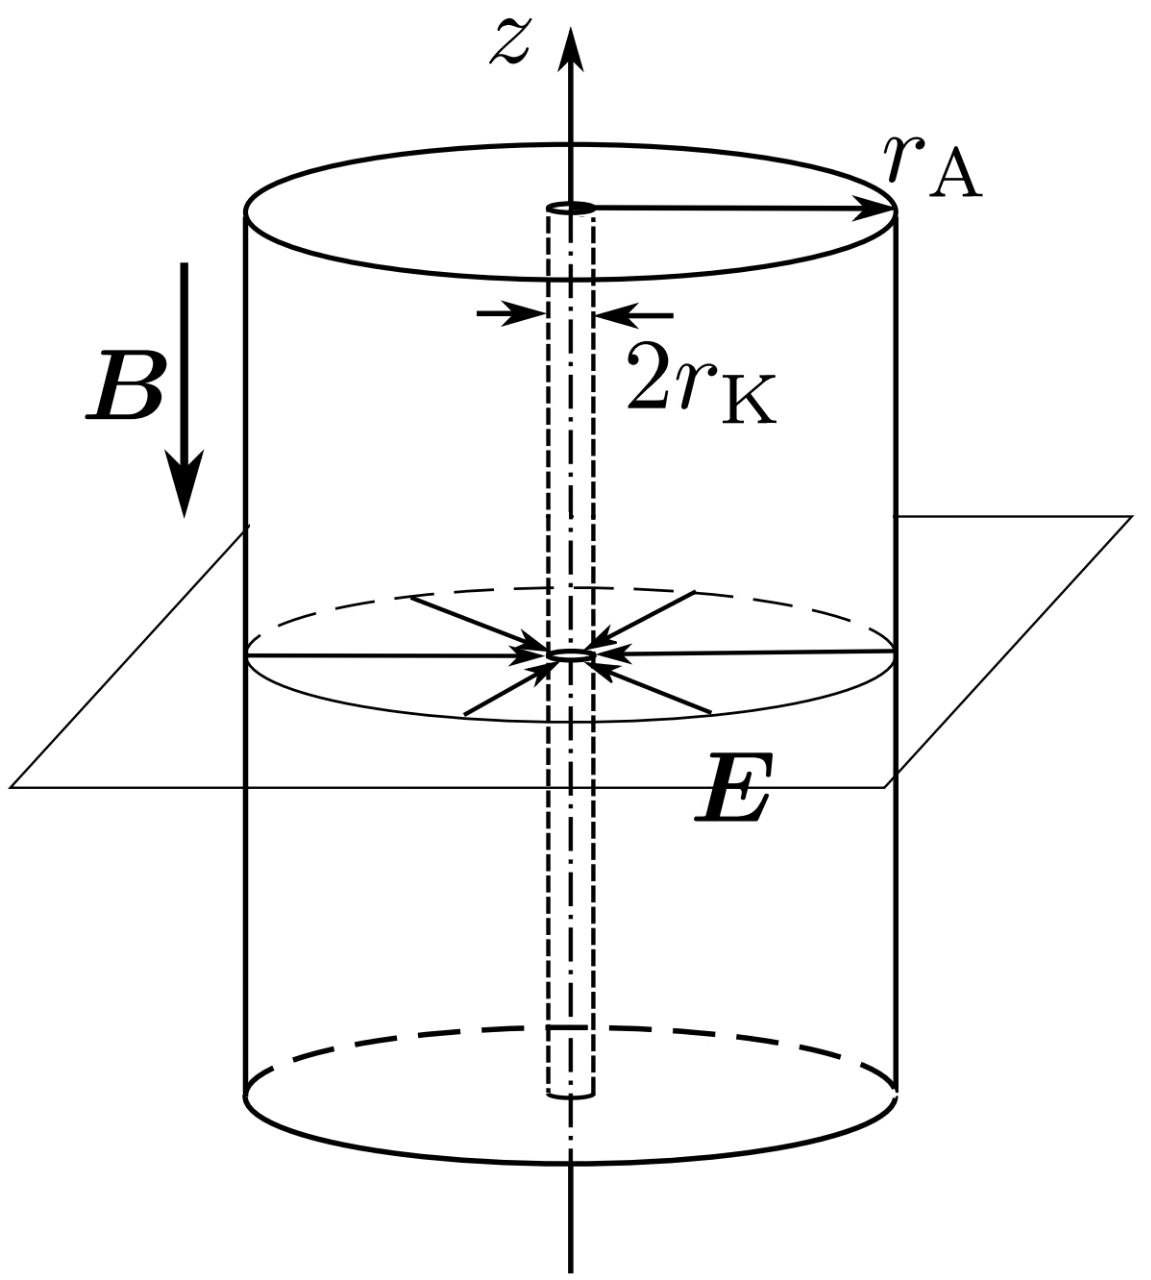
\includegraphics[width = 0.5\textwidth]{СхемаДвухЭлектроднойЛабы}
\caption{Двухэлуктродная лампа}
\label{2elbulb}
\end{center}
\end{figure}

В данной работе движение электронов происходит в кольцевом про­странстве, ограниченном катодом и анодом двухэлектродной электрон­ной вакуумной лампы (\hyperref[2elbulb]{fig. 6}). Нить накала лампы (катод) располагается вдоль оси цилиндрического анода, так что электрическое поле между катодом и анодом имеет радиальное направление. Лампа помещается внутри соленоида, создающего магнитное поле, параллельное оси лам­пы.
Таким образом, реализуется геометрия скрещенных полей $E$ и $B$.
%Поскольку поле $E$ в данном случае не является однородным (оно зависит от расстояния до оси), траектории частиц будут несколько отличаться от рассмотренного выше плоского случая. Тем не менее все качественные особенности траектории сохранятся, а выражение для критического поля будет отличаться от \hyperref[RivMass]{(\ref{RivMass})} только численным коэффициентом порядка единицы.\\

\begin{figure}[h]
	\begin{center}
		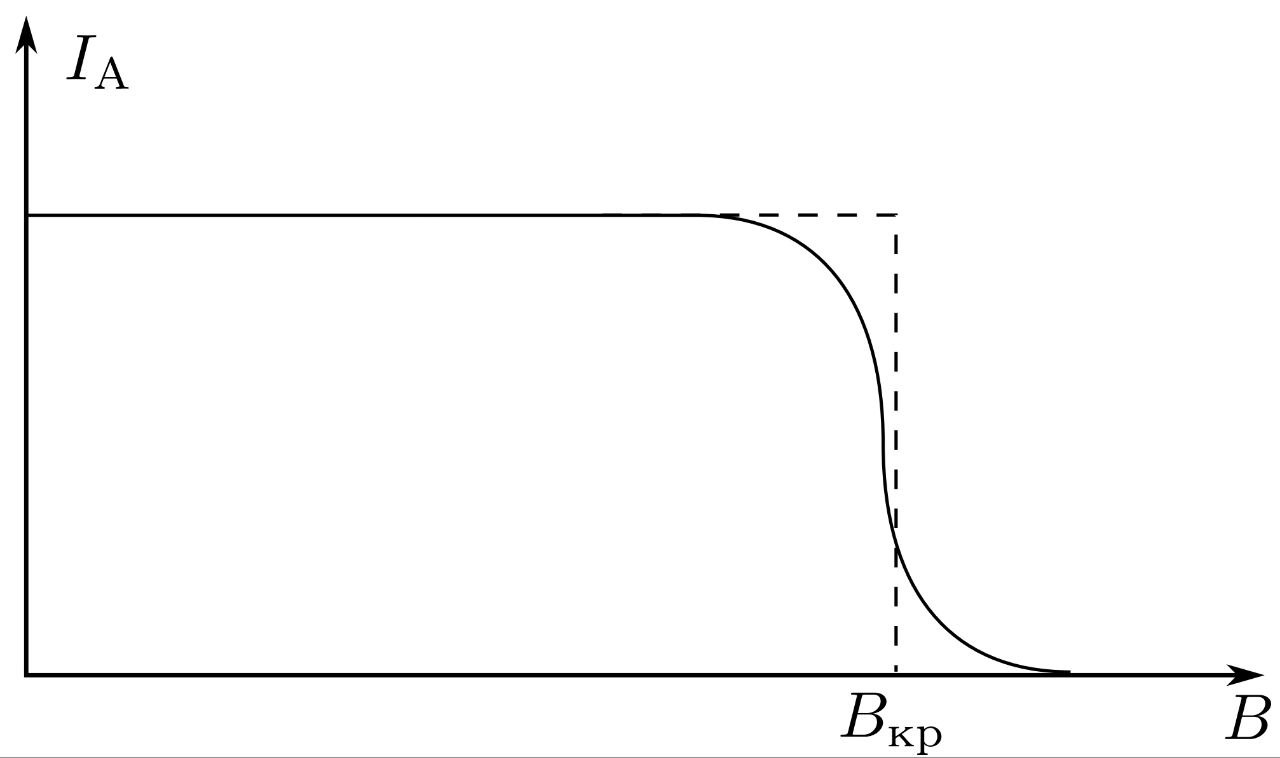
\includegraphics[width = \textwidth]{ЗависимостьТокаотМагнПоля}
		\caption{Зависимость анодного тока от индукции магнитного поля в соленоиде}
	\end{center}
\label{IA(B)}
\end{figure}

До сих пор мы рассматривали идеальный случай: при $B<B_{\text{кр}}$ все электроны без исключения попадают на анод, а при $B > B_{\text{кр}}$ все они возвращаются на катод, не достигнув анода. Анодный ток $I_A$ с увеличением магнитного поля изменялся бы при этом так, как это изображено штриховой линией на \hyperref[IA(B)]{fig. 7}. В реальных условиях невозможно обеспечить полную коаксиальность анода и катода, вектор индукции магнитного поля всегда несколько наклонён по отношению к катоду, магнитное поле не вполне однородно и т. д. Всё это приводит к сглаживанию кривой $I_A(B)$ (\hyperref[IA(B)]{fig. 7}). Однако в хорошо собранной установке перелом функции $I_A(B)$ остаётся достаточно резким и может быть использован для измерения $\frac{e}{m}$. Схема установки изображена на \hyperref[MethMagnetron]{fig. 8}. Анод лампы состоит из трёх немагнитных металлических цилиндров одинакового диаметра. Два крайних цилиндра электрически изолированы от среднего неболь­шими зазорами и используются для устранения краевых эффектов на торцах среднего цилиндра, ток с которого используется при измерени­ях. В качестве катода используется тонкая (диаметр $2r_K = 50$ мкм) натянутая вольфрамовая проволока, расположенная по оси всех трёх цилиндров анодной системы. Катод разогревается проходящим через него переменным током (лампа прямого накала), создаваемым стабилизиро­ванным источником питания. На анод лампы подаётся постоянное напря­жение от регулируемого источника, измеряемое вольтметром $V_A$. Ток $I_A$ через среднюю секцию анода измеряется с помощью миллиамперметра.\\
Лампа закреплена в соленоиде. Ток $I_C$, проходящий через соленоид, подаётся от независимого источника и измеряется амперметром. Индук­ция магнитного поля в соленоиде рассчитывается по току, протекающе­му через обмотку соленоида.

\begin{figure}[h]
	\begin{center}
		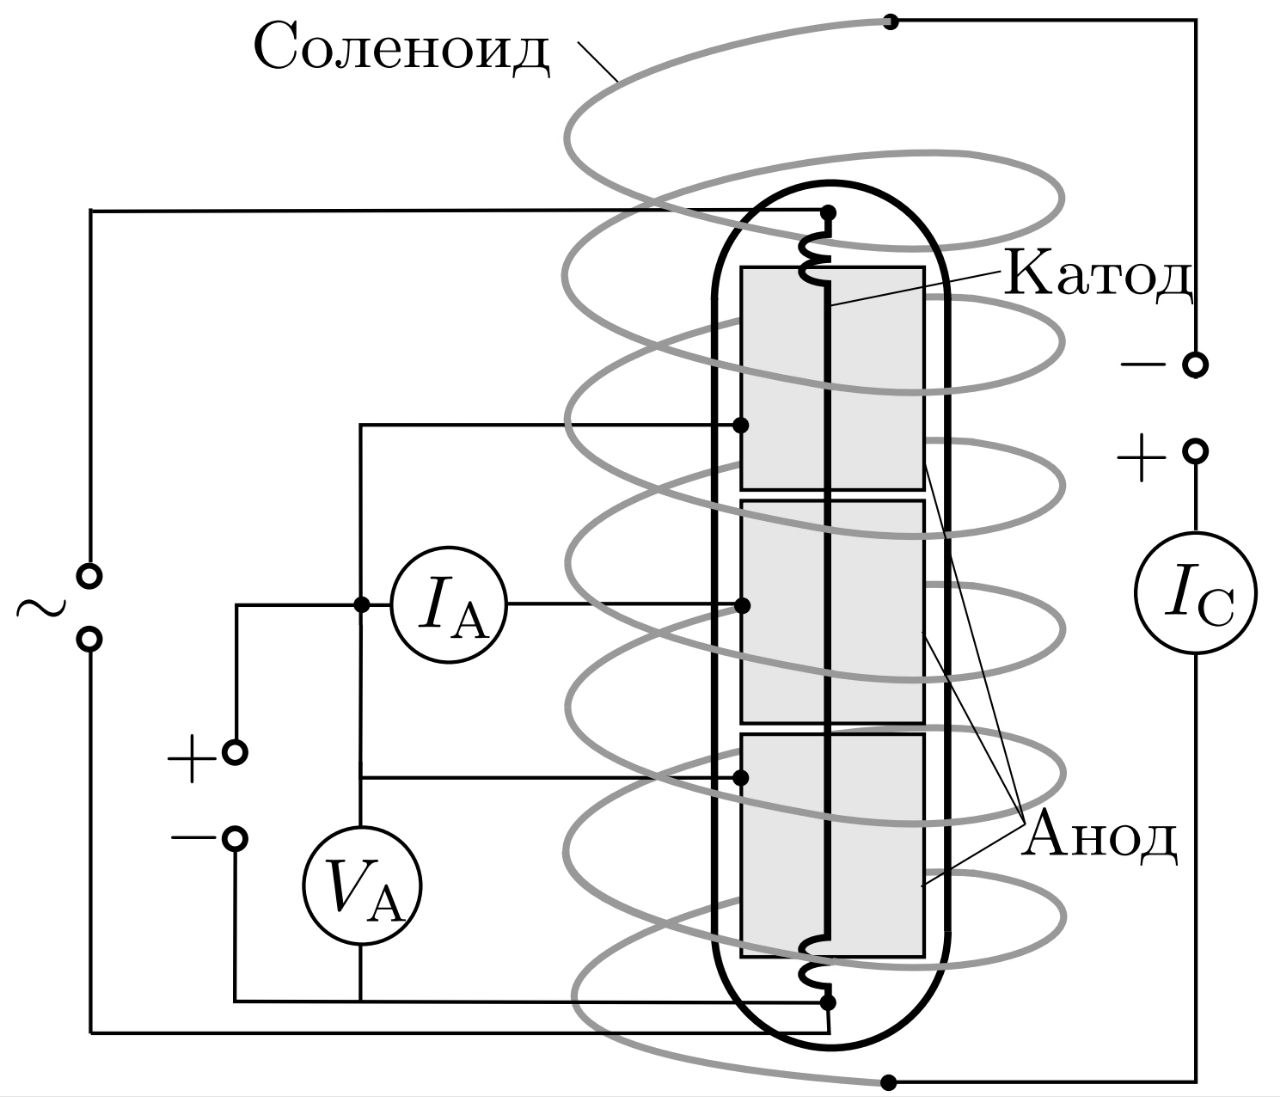
\includegraphics[width = 0.5\textwidth]{Метод2}
		\caption{Измерительная установка}
	\end{center}
\label{MethMagnetron}
\end{figure}

\subsection*{Эксперементальные данные}

\begin{table}[h]
\begin{center}
\begin{tabular}{|c|c|c|c|c|c|c|c|c|c|}
\hline 
\multicolumn{2}{|c}{$V_A = 70$ В} & \multicolumn{2}{|c}{$V_A = 80$ В} & \multicolumn{2}{|c}{$V_A = 90$ В} & \multicolumn{2}{|c}{$V_A = 100$ В} & \multicolumn{2}{|c|}{$V_A = 110$ В} \\ 
\hline
\multicolumn{2}{|c}{$I_A: 150\text{дел} = 0.3A$} & \multicolumn{8}{|c|}{$I_A: 150\text{дел} = 0.6A$}\\
\multicolumn{2}{|c}{$I_A: 75\text{дел} = 1.5A$} & \multicolumn{8}{|c|}{$I_A: 75\text{дел} = 1.5A$}\\
\hline 
$I_c,$ дел & $I_A,$ дел & $I_c,$ дел & $I_A,$ дел & $I_c,$ дел & $I_A,$ дел & $I_c,$ дел & $I_A,$ дел & $I_c,$ дел & $I_A,$ дел \\ 
\hline 
5.5 & 142 & 1.0 & 117 & 1.0 & 114 & 1.0 & 109 & 1.0 & 110 \\ 
\hline 
6.5 & 81 & 2.0 & 113 & 3.0 & 108 & 3.0 & 108 & 3.0 & 110 \\ 
\hline 
7.0 & 60 & 3.0 & 110 & 5.0 & 94 & 4.0 & 107 & 4.0 & 109 \\ 
\hline 
7.5 & 17 & 4.0 & 100 & 6.0 & 84 & 5.0 & 98 & 5.0 & 100 \\ 
\hline 
8.0 & 12 & 5.0 & 87 & 7.0 & 62 & 6.0 & 94 & 5.5 & 100 \\ 
\hline 
9.0 & 6 & 6.0 & 68 & 7.5 & 45 & 6.5 & 88 & 6.0 & 100 \\ 
\hline 
\multicolumn{2}{|c|}{} & 7.0 & 35 & 8.0 & 31 & 7.0 & 78 & 7.0 & 92 \\ 
\cline{3-10} 
\multicolumn{2}{|c|}{} & 7.5 & 13 & 8.5 & 13 & 7.5 & 69 & 8.0 & 75 \\ 
\cline{3-10}
\multicolumn{2}{|c|}{} & 8.0 & 7 & 9.0 & 7 & 8.0 & 62 & 8.5 & 64 \\ 
\cline{3-10}
\multicolumn{2}{|c|}{} & 8.5 & 5 & 9.5 & 5 & 8.5 & 44 & 9.0 & 42 \\ 
\cline{3-10}
\multicolumn{2}{|c|}{} & 9.0 & 3 & 10.0 & 4 & 9.0 & 15 & 9.5 & 32 \\ 
\cline{3-10}
\multicolumn{2}{|c|}{} & 10.0 & 2 & \multicolumn{2}{c|}{} & 9.5 & 10 & 10.0 & 8 \\ 
\cline{3-4} \cline{7-10}
\multicolumn{6}{|c|}{} & 10.0 & 6 & 11.0 & 5 \\ 
\hline
\end{tabular} 
\caption{зависимость анодного тока $I_A$ от тока через соленоид $I_C$}
\end{center}
\end{table}

По данным таблицы сторим зависимости $I_A$ от $B$ при разных $V$.
\[B = K * I_c,~\text{где}~K = 2.8 \cdot10^{-2}\frac{\text{Тл}}{\text{A}}\]

\begin{figure}[h]
	\begin{center}
		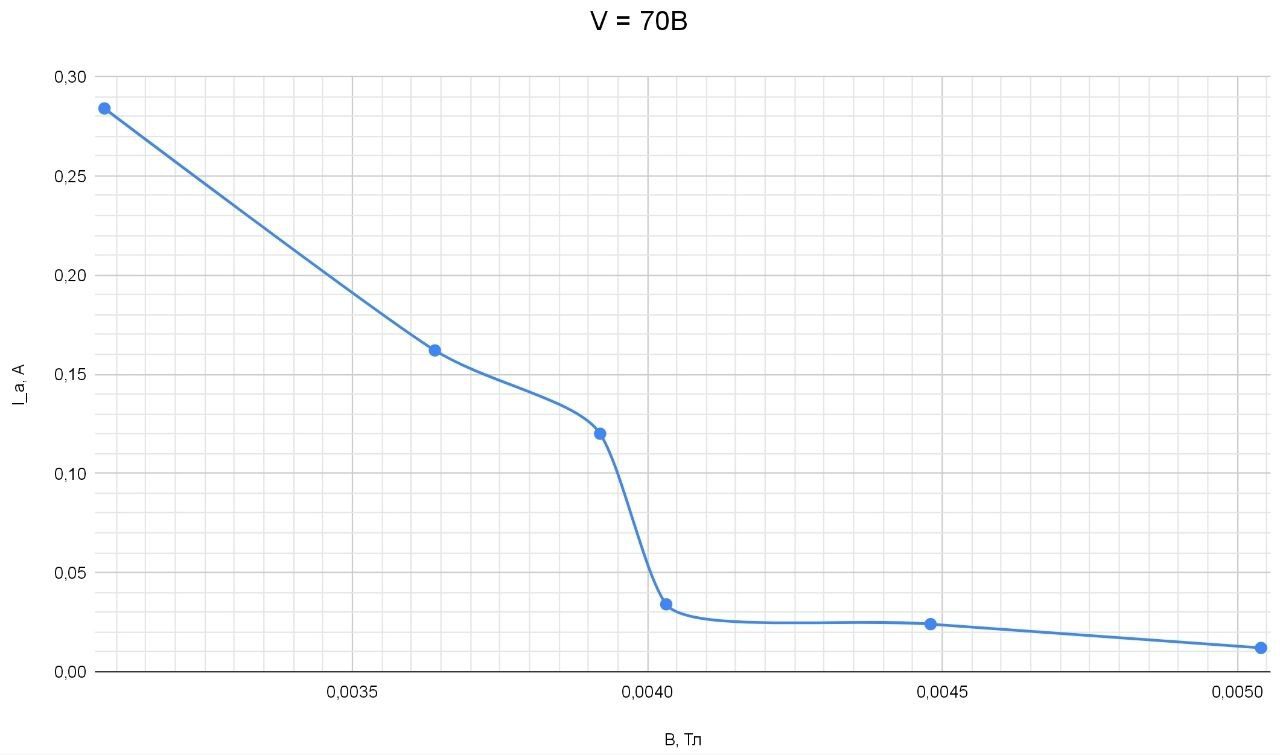
\includegraphics[width = 0.78\textwidth]{V70B}
		\caption{$I_A$ от $B$ при V = 70 B}
	\end{center}
\end{figure}

\begin{figure}[h]
	\begin{center}
		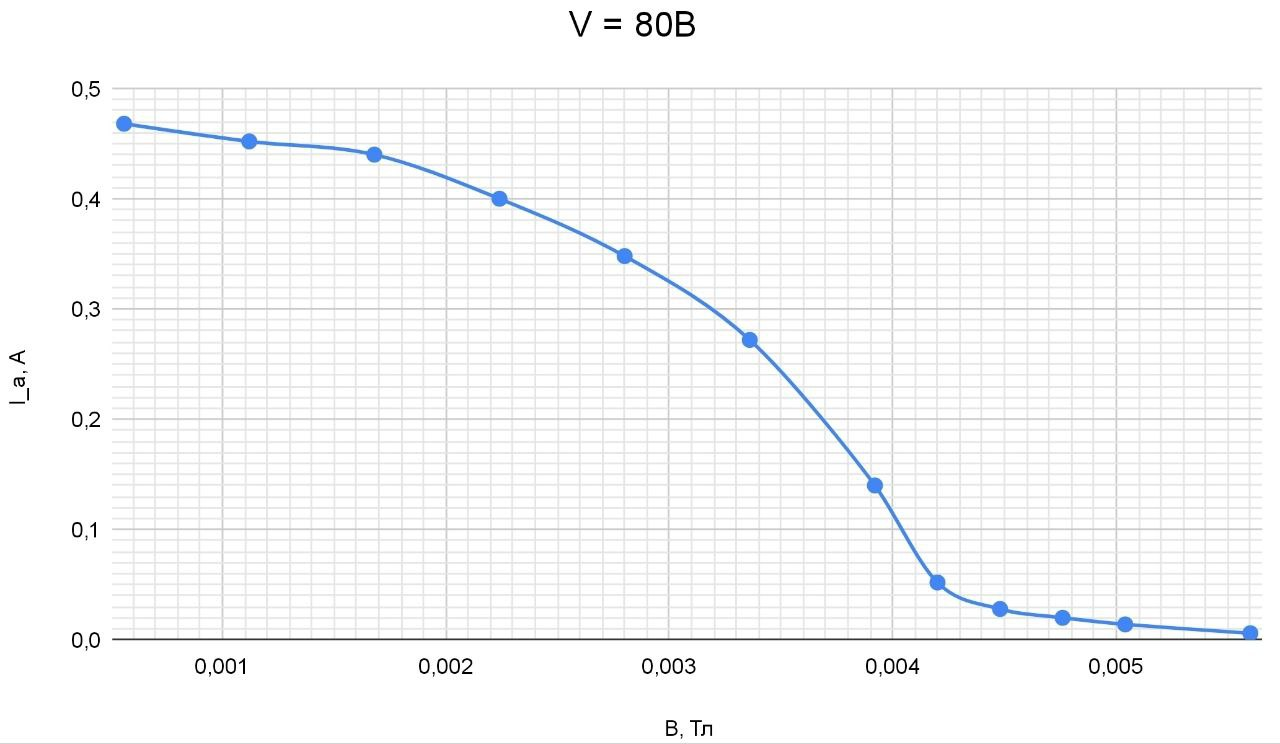
\includegraphics[width = 0.78\textwidth]{V80B}
		\caption{$I_A$ от $B$ при V = 80 B}
	\end{center}
\end{figure}

\begin{figure}[h]
	\begin{center}
		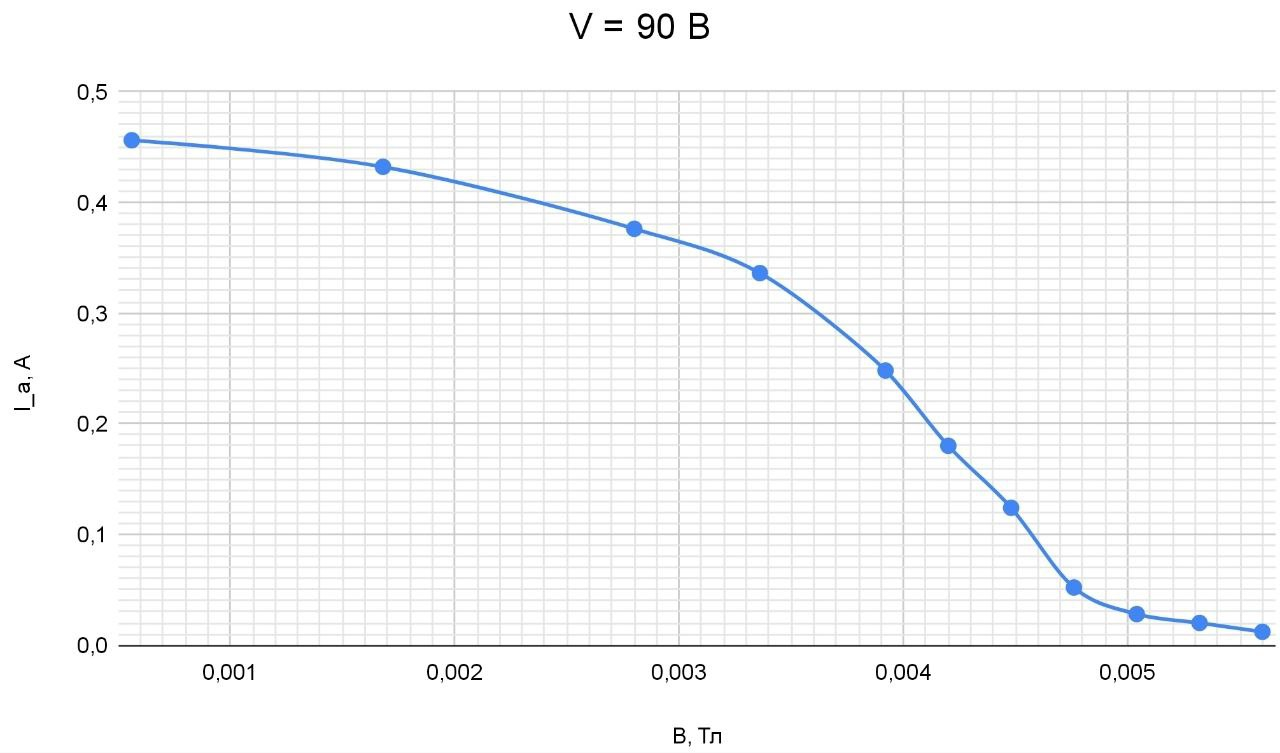
\includegraphics[width = 0.78\textwidth]{V90B}
		\caption{$I_A$ от $B$ при V = 90 B}
	\end{center}
\end{figure}

\begin{figure}[h]
	\begin{center}
		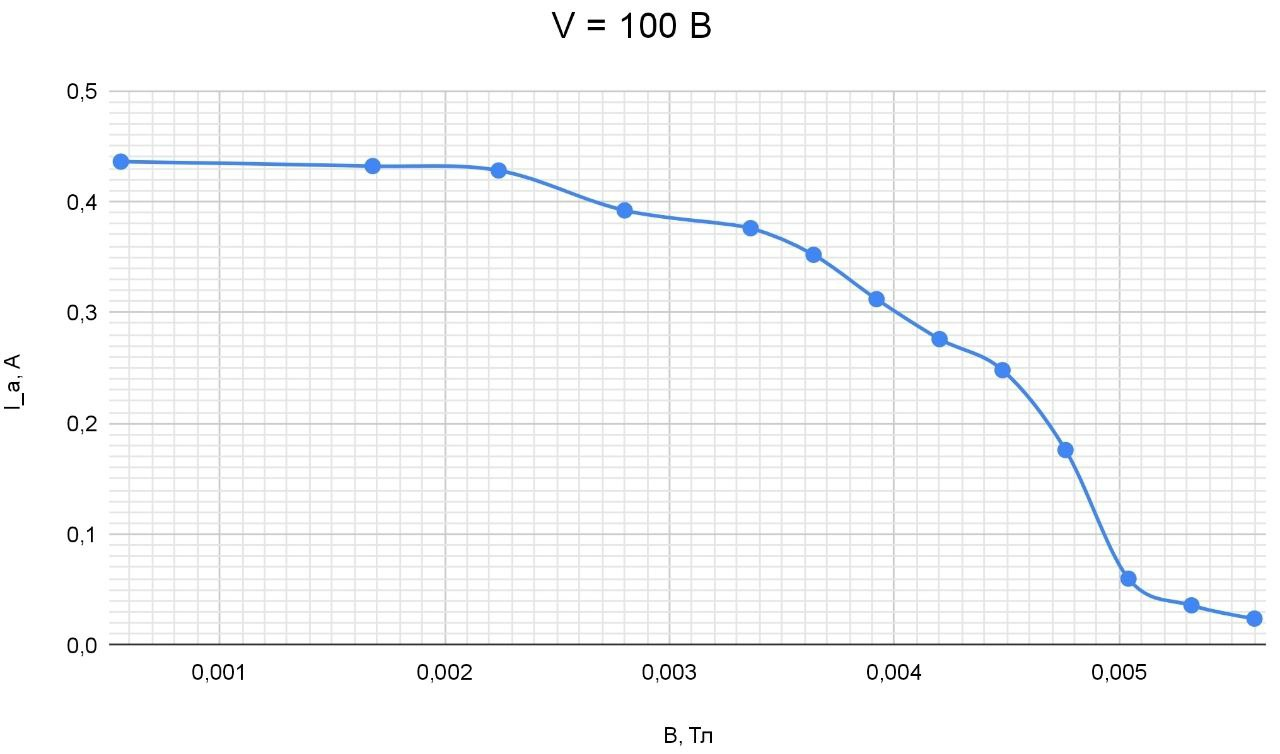
\includegraphics[width = 0.78\textwidth]{V100B}
		\caption{$I_A$ от $B$ при V = 100 B}
	\end{center}
\end{figure}

\begin{figure}[h]
	\begin{center}
		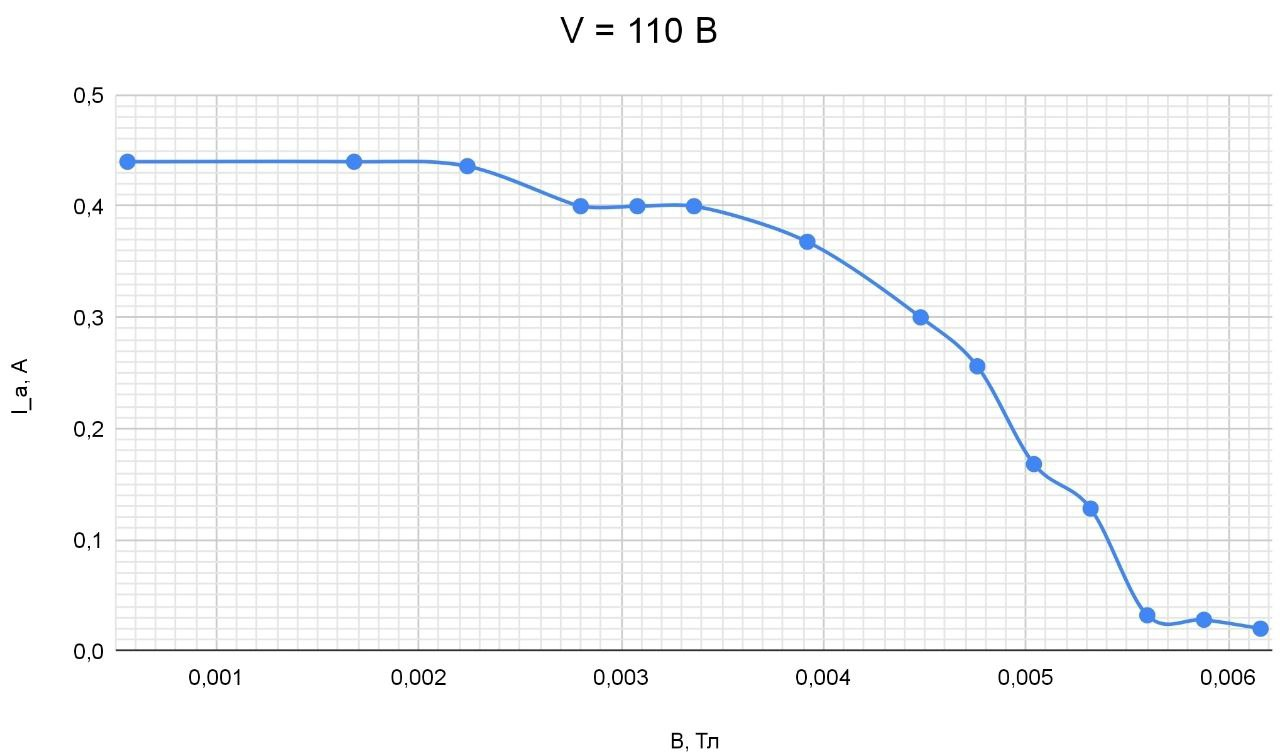
\includegraphics[width = 0.78\textwidth]{V110B}
		\caption{$I_A$ от $B$ при V = 110 B}
	\end{center}
\end{figure}

Из графиков находим $B_\text{кр}$ для разных значений $V$ и сторим график зависимости $B_\text{кр}^2$ от $V$.

\begin{figure}[h]
	\begin{center}
		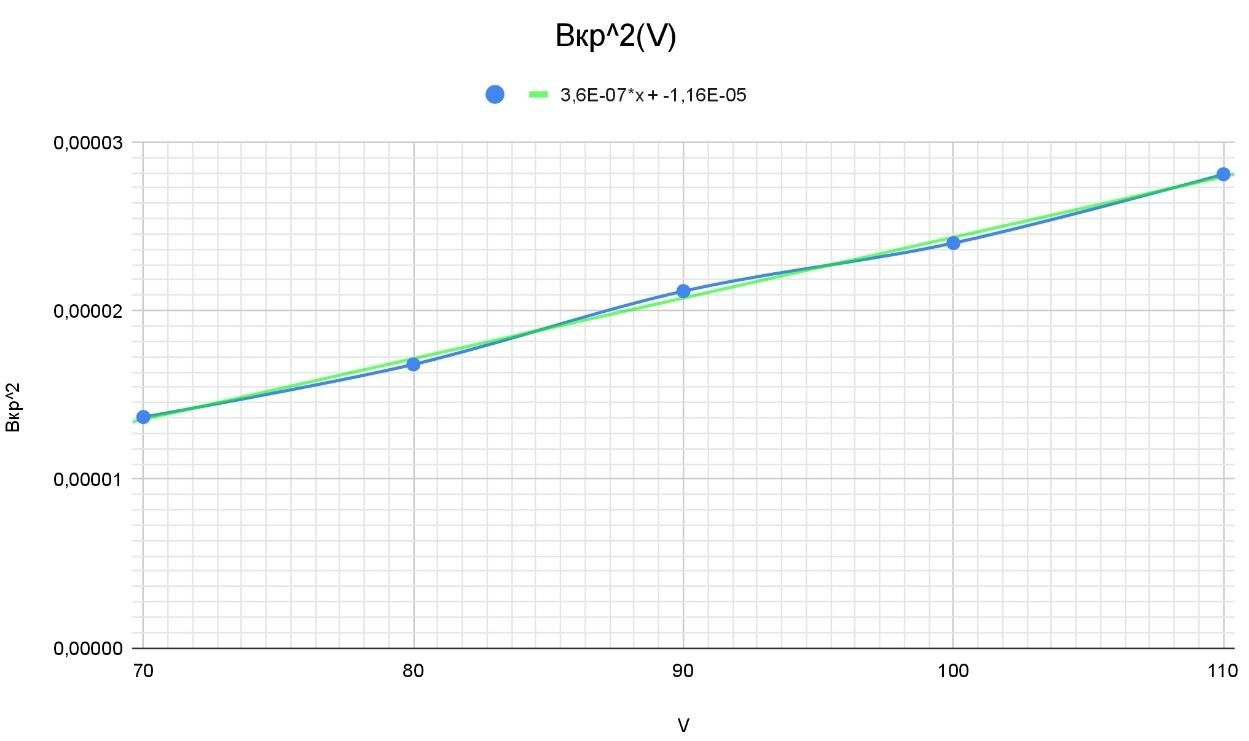
\includegraphics[width = 0.78\textwidth]{Bкр(V)}
		\caption{Зависимость $B_\text{кр}^2$ от $V$}
	\end{center}
\end{figure}

Из этого графика получаем коэффициент наклона прямой: $q = 3.59 \cdot 10^{-7}$.\\
Находим $\frac{e}{m}$ по формуле \ref{RealMsss}:
\[\frac{e}{m} = \frac{8}{q r_A^2} = \frac{8}{3.2\cdot10^{-7}\times \left(12\cdot10^{-3}\right)^2} \approx1.74 \cdot10^{11}\]

\section*{Вывод}
Полученные значения примерно равны друг другу и приблизительно равны табличному ($1.55 \cdot 10^{11}$), вклад в погрешность, кроме систематических, также давала неточность определения $B_\text{кр}$.

\clearpage
\listoffigures
\listoftables

\end{document}
